\documentclass[conference]{IEEEtran}
\IEEEoverridecommandlockouts

\usepackage{cite}
\usepackage{amsmath,amssymb,amsfonts}
\usepackage{graphicx}
\usepackage{booktabs}
\usepackage{url}
\usepackage{balance}
\usepackage[caption=false,font=footnotesize]{subfig}

\graphicspath{{figures/}}

\def\BibTeX{{\rm B\kern-.05em{\sc i\kern-.025em b}\kern-.08em
    T\kern-.1667em\lower.7ex\hbox{E}\kern-.125emX}}

\begin{document}

\title{Measuring the Cost of Xn Handover in Non-Terrestrial Networks:\\
An Emulation Study Driven by Real LEO Ephemeris}

\author{\IEEEauthorblockN{Author Name}
\IEEEauthorblockA{\textit{Department} \\
\textit{Institution}\\
City, Country \\
email@institution.edu}
}

\maketitle

\begin{abstract}
Handover studies for non-terrestrial networks (NTN) almost universally count
handovers, treating each as a cost-free event. This obscures a term that
matters: handovers differ substantially in what they cost, and the policies
that minimise handover \emph{count} systematically select the most expensive
ones. We present an emulation testbed in which real 3GPP Xn handovers are
executed between software gNBs while propagation delays derived from actual
Starlink ephemeris are injected on individual 5G interfaces. Across 470 measured
handovers we decompose handover latency into its signalling and core-processing
components and quantify, for the first time to our knowledge, how much
user-plane interruption a millisecond of delay on each link actually buys.
We find a strong asymmetry: delay on the inter-satellite Xn link inflates
handover latency ($+0.46$\,ms/ms) but contributes essentially \emph{zero}
interruption ($-0.01$\,ms/ms), because it is paid before the UE leaves the
source cell, whereas feeder- and service-link delay convert almost directly into
downtime ($+0.80$ and $+1.24$\,ms/ms). Replaying real satellite pass sequences,
we show that a maximum-elevation policy performs $7\times$ more handovers than a
maximum-service-time policy but each costs only half as much
($9.55$ vs.\ $19.47$\,ms), so the $7\times$ count advantage reduces to
$3.4\times$ in cumulative interruption. Counting handovers therefore overstates
the benefit of stability-focused policies, because the handovers they avoid are
the cheap ones.
\end{abstract}

\begin{IEEEkeywords}
non-terrestrial networks, LEO satellite, Xn handover, 5G, handover
interruption, mobility management, testbed
\end{IEEEkeywords}

\section{Introduction}

Low Earth Orbit (LEO) constellations move fast enough that a satellite serves a
given ground user for only a few minutes, making mobility management a dominant
concern in non-terrestrial networks. A large literature accordingly compares
satellite-selection policies---maximum elevation, maximum remaining service
time, maximum SINR, and hybrids---and reports how many handovers each incurs
\cite{ref_hybrid,ref_demand,ref_optimal,ref_graph}.

That body of work shares a modelling assumption: a handover is an instantaneous
event whose only cost is that it happened. In a real 5G system a handover is a
multi-message procedure spanning the radio interface, the inter-base-station
interface, and the core network, and its duration depends on the propagation
delay of the links it traverses. Under NTN geometry those delays vary by more
than a factor of three across a single satellite pass. A policy that chooses
\emph{when} to hand over is therefore also choosing \emph{how expensive} that
handover will be---a coupling that count-based studies cannot express.

This paper measures that coupling. Our contributions are:

\begin{itemize}
\item An emulation testbed that performs standards-conformant 3GPP Xn handovers
between software gNBs, with per-link propagation delay injected from real
Starlink ephemeris (Sections~\ref{sec:testbed}--\ref{sec:ntn}).
\item A decomposition of handover cost showing that \emph{where} delay sits
determines whether it causes interruption. Xn-link delay costs latency but not
downtime; feeder- and service-link delay cost both (Section~\ref{sec:e2}).
\item A live replay of real pass sequences establishing that per-handover cost
is inversely related to handover frequency, which materially changes the
policy trade-off reported in the literature (Section~\ref{sec:e4}).
\end{itemize}

\section{Background}

\subsection{Xn Handover in 3GPP}

In an Xn handover the source and target gNBs communicate directly rather than
routing the procedure through the core \cite{ref_38300}. The sequence is:
(i)~the source sends a \emph{Handover Request} carrying the UE context over Xn;
(ii)~the target admits the UE and acknowledges; (iii)~the source sends the UE an
\texttt{RRCReconfiguration} containing \texttt{reconfigurationWithSync}---the
handover command~\cite{ref_38331}; (iv)~the UE synchronises to the target and
replies
\texttt{RRCReconfigurationComplete}; (v)~the target sends a \emph{Path Switch
Request} to the AMF, which redirects the downlink tunnel via the SMF and UPF;
(vi)~the target releases the source context.

Two properties matter here. The path switch occurs \emph{after} the UE has
arrived, not before, so the core is only asked to move the tunnel once the UE is
reachable at the target. And for an intra-AMF, intra-tracking-area handover the
UE remains RRC-CONNECTED throughout, so no NAS signalling is generated.

Baseline 3GPP handover is \emph{break-before-make}: the UE stops using the
source before it starts using the target, and a short user-plane gap is
expected. Reference interruption times are $\geq$45\,ms for LTE and 24\,ms
(FR1) / 7.4\,ms (FR2) for NR with a make-before-break configuration
\cite{ref_daps}. Dual Active Protocol Stack (DAPS) handover, introduced in
Rel-16, targets near-zero interruption but is \emph{explicitly not supported for
NTN}, as maintaining simultaneous connections to two satellites is impractical
given payload and feeder-link constraints \cite{ref_ntnproc}. NTN instead relies
on RACH-less handover and conditional handover with NTN-specific triggers.

\subsection{Mobility Triggers in NTN}

3GPP defines no elevation-angle event. The NTN-specific Rel-17 conditional
handover conditions are \textsc{CondEvent~D1} (distance to the serving cell
reference location above one threshold and distance to the candidate below
another) and \textsc{CondEvent~T1} (a time window) \cite{ref_ntnproc}. Because
elevation angle and slant range are monotonically related, an elevation
threshold is equivalent to a D1-style distance condition, and a
remaining-service-time criterion is a T1-style time condition. We use elevation
throughout for interpretability while noting this correspondence.

We emphasise that the mechanism studied here is \emph{elevation-triggered
handover}, not conditional handover: the network evaluates the condition and
issues a command. In true CHO the UE holds candidate configurations and
evaluates the conditions autonomously.

\section{Testbed}
\label{sec:testbed}

\subsection{Architecture}

The testbed comprises an Open5GS~\cite{ref_open5gs} 5G core and a modified
UERANSIM~\cite{ref_ueransim} radio-access simulator, with three software gNBs and one UE. All gNBs register to the same
AMF with a common tracking area and slice identifier, since an Xn path switch is
only meaningful when source and target are served by the same AMF.
Table~\ref{tab:testbed} summarises the configuration.

\begin{table}[t]
\caption{Testbed configuration}
\label{tab:testbed}
\centering
\begin{tabular}{ll}
\toprule
Component & Configuration \\
\midrule
Core network & Open5GS (AMF, SMF, UPF, and support NFs) \\
RAN & UERANSIM with Xn handover extension \\
gNBs & 3, common PLMN / TAC / S-NSSAI, one AMF \\
UE & 1, single PDU session, isolated namespace \\
Delay injection & per-interface, per-gNB \\
Ephemeris & Starlink TLE, Montreal ground station \\
\bottomrule
\end{tabular}
\end{table}

\subsection{Xn Handover Procedure}

UERANSIM does not natively implement inter-gNB mobility. We added a complete Xn
handover following the 3GPP ordering described above. The source gNB transfers
the UE context---security parameters, PDU session tunnel endpoints and QoS flow
identifiers---to the target over a dedicated Xn interface. The target admits the
UE and holds the context in a pending state. The source then issues a genuine
\texttt{RRCReconfiguration} carrying \texttt{reconfigurationWithSync}, which
identifies the target cell; it does \emph{not} release the UE. On receiving the
command the UE re-points its serving cell, remains RRC-CONNECTED, and replies
\texttt{RRCReconfigurationComplete} to the target. Only then does the target
issue the NGAP \emph{Path Switch Request}, and only on acknowledgement does it
instantiate the user-plane tunnels.

Three design points are worth stating because they determine what the
measurements mean. First, the path switch is deferred until the UE has actually
arrived, so a handover the UE never completes never reaches the core. Second,
source and target correlate the UE through an identifier the UE itself
generates and both gNBs already possess, so the context created by the path
switch \emph{is} the context the UE is connected through---there is no second,
orphaned context. Third, the UE never enters idle, so no NAS re-registration
occurs; this is verified in every run by the absence of registration signalling.

We do not implement SN Status Transfer or a data-forwarding tunnel, so the
procedure is not lossless; a brief user-plane gap is expected and is precisely
the quantity we measure.

\subsection{Isolation of the Data Path}

A subtlety with material consequences: when the UE and the core share a network
namespace, the UE's IP address is local to the host, and the kernel's local
routing table short-circuits every downlink packet to a local socket. Downlink
then never traverses the GTP tunnel, and any user-plane measurement is
meaningless while appearing to succeed. We therefore run the UE in an isolated
network namespace, which forces downlink through the full
UPF~$\rightarrow$~GTP~$\rightarrow$~gNB~$\rightarrow$~radio path. The
distinction is visible in round-trip time: ${<}0.1$\,ms when short-circuited
versus 1--6\,ms through the real path.

\section{NTN Modelling}
\label{sec:ntn}

\subsection{Geometry}

Satellite positions are propagated with SGP4~\cite{ref_skyfield} from real
Starlink two-line elements over a ground station at Montreal ($45.5017^\circ$\,N,
$73.5673^\circ$\,W). Two choices preserve fidelity. Passes are computed at the
TLE \emph{epoch} rather than at wall-clock time, since a TLE is accurate only
for a few days around its epoch. And only satellites within the 500--600\,km
operational shell are considered, because the element set also contains lowered
and de-orbiting satellites whose geometry would understate a representative LEO
link.

The selected reference pass (STARLINK-3075, $87^\circ$ culmination) spans slant
ranges of 544--1805\,km, giving one-way propagation delays of
1.82--6.02\,ms. Fig.~\ref{fig:geo} shows delay against elevation with the
sweep points marked. Over a one-hour window the constellation presents 270
passes with a median duration of 7.4 minutes and up to 43 satellites
simultaneously visible above $10^\circ$.

\begin{figure}[t]
\centering
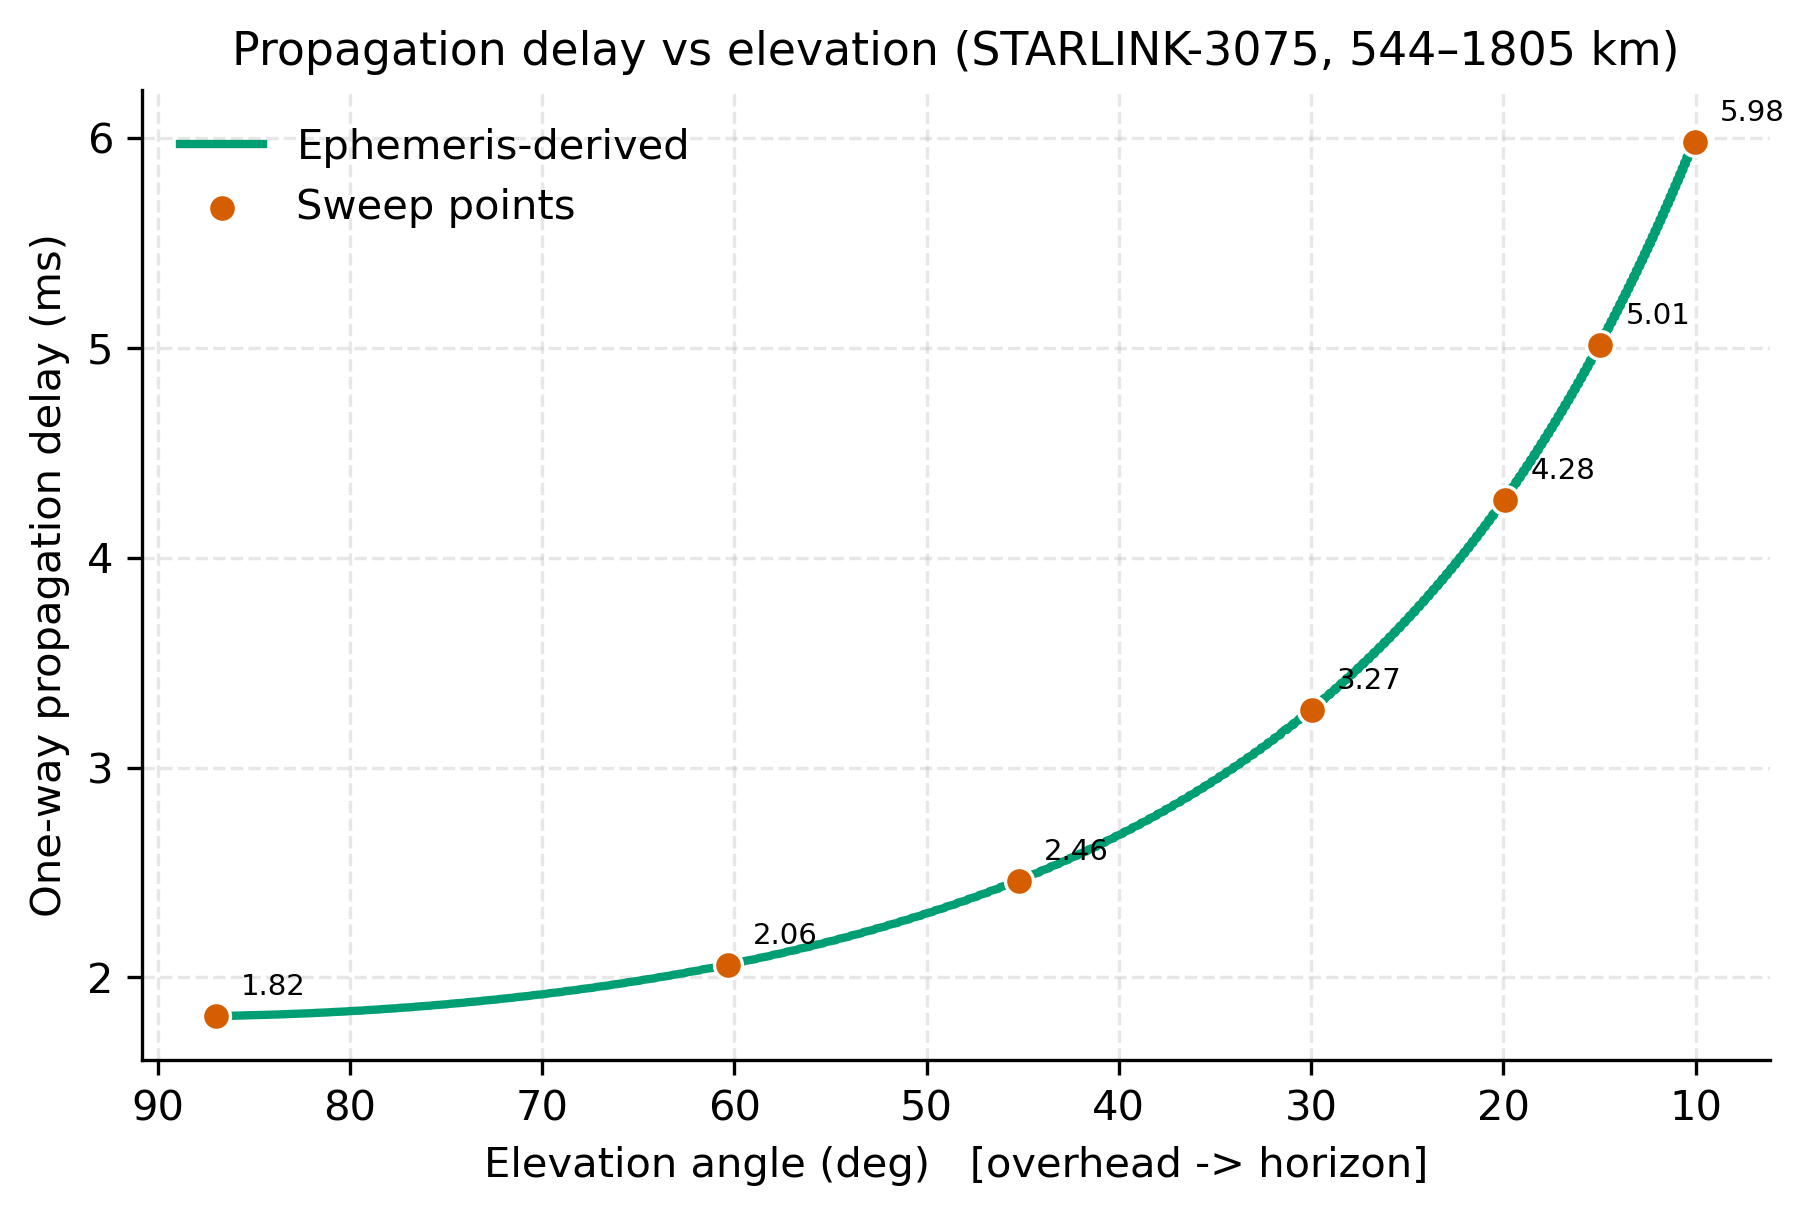
\includegraphics[width=\columnwidth]{fig_geo_elevation.png}
\caption{One-way propagation delay against elevation angle, derived from real
Starlink ephemeris over Montreal. Markers indicate the operating points used in
the delay sweep.}
\label{fig:geo}
\end{figure}

\subsection{Delay Injection and Architecture Scenarios}

Propagation delay is injected independently on each 5G interface using kernel
traffic shaping, applied at both ends of every link so that each side carries
the one-way delay and the round trip emerges naturally. Jitter is deliberately
not used: it reorders packets, which propagation delay does not, and would
corrupt the interruption measurement.

Which interface carries the long delay depends on payload architecture, giving
three scenarios (Table~\ref{tab:scenarios}). Under a \emph{transparent} payload
the satellite is a bent-pipe relay and the gNB is on the ground, so the service
and feeder hops together form the radio link. Under a \emph{regenerative}
payload the gNB is aboard the satellite, so the feeder link to the ground
carries N2 and N3. When source and target gNBs are on different satellites, the
\emph{inter-satellite} link carries Xn.

\begin{table}[t]
\caption{NTN architecture scenarios}
\label{tab:scenarios}
\centering
\begin{tabular}{lll}
\toprule
Scenario & gNB location & Long link \\
\midrule
Transparent & Ground & Radio (service + feeder) \\
Regenerative & On satellite & Feeder (N2 + N3) \\
Inter-satellite & Two satellites & Xn \\
\bottomrule
\end{tabular}
\end{table}

\subsection{Handover Policies}

Three satellite-selection policies from the LEO literature are implemented.
\emph{Maximum elevation} always serves on the highest-elevation visible
satellite. \emph{Elevation threshold} holds the serving satellite until its
elevation falls below a threshold. \emph{Maximum remaining service time} holds
until the serving satellite is close to setting, then selects the candidate with
the longest remaining visibility.

All three apply the stability controls that make a trigger usable in practice: a
hysteresis margin, so a candidate must exceed the serving cell by a margin
rather than merely exceed it; a time-to-trigger, so the condition must hold
continuously; a minimum dwell time between handovers; and a lead time, so the
handover completes before the serving link becomes unusable. The lead time is
the direct coupling between measured handover cost and policy design.

\section{Experimental Design}

\subsection{Metrics}

Each handover yields three latency components measured by the target gNB with
microsecond-resolution timestamps:

\begin{itemize}
\item \textbf{UE arrival} --- from the Xn Handover Request arriving at the
target to the UE completing its move. Covers Xn signalling, handover command
delivery, and the radio switch.
\item \textbf{Path switch} --- from Path Switch Request to Acknowledge. This is
core processing: AMF, SMF and UPF updating the tunnel.
\item \textbf{Total} --- the whole procedure at the target.
\end{itemize}

User-plane interruption is measured with a high-rate probe traversing the GTP
tunnel throughout each handover. The outage is computed as the number of
\emph{contiguous} missing probes multiplied by the inter-arrival spacing
\emph{actually achieved}. Both halves matter: the contiguous count isolates the
handover from unrelated scattered loss, while the achieved spacing is required
because probe pacing degrades toward the round-trip rate once delay is injected.
Measurement resolution is consequently one probe interval, 1.2\,ms undelayed
and 5--8\,ms under injected delay.

\subsection{Experimental Controls}

Two effects were identified during validation that would otherwise confound the
results, and both are controlled.

\emph{Handover cadence affects core processing.} At 2.2\,s between handovers the
path-switch time nearly doubles relative to 5\,s, as the core does not settle
between procedures. Every configuration therefore uses a fixed cycle period so
the core sees an identical handover rate throughout.

\emph{Probe traffic perturbs the measurement.} At 1000 probes per second the
measurement traffic queues behind the delayed link and inflates the measured
path-switch time. This is quantified in Section~\ref{sec:e2} and bounds the
precision of one reported coefficient.

Each measurement session is bracketed by identical baseline runs to detect
drift. Across a full session the baseline moved from 3.897\,ms to 4.087\,ms
median path-switch time, confirming stability.

\subsection{Experiments}

\textbf{E1} establishes the zero-delay baseline (50 handovers).
\textbf{E2} sweeps the seven elevation operating points for each of the three
architecture scenarios, 20 handovers per point (420 total).
\textbf{E3} evaluates the three policies offline against the real constellation
schedule, isolating decision behaviour from execution cost.
\textbf{E4} replays real pass sequences against the live testbed: each gNB's
service-link delay tracks whichever satellite it currently represents, and a
real Xn handover fires when the policy dictates. Four independent 15-minute
windows are used per policy. Because only two gNBs are needed---the freed gNB is
reassigned to the next satellite after each handover---arbitrarily long pass
chains are supported. Geometry is replayed on an accelerated clock, which is
sound because geometry evolves over minutes while a handover completes in
milliseconds; the handovers themselves execute in real time.

\section{Results}

\subsection{Baseline}

Over 50 handovers with no injected delay the procedure completes in a median of
4.744\,ms (mean $4.891 \pm 0.664$\,ms), decomposing into 0.831\,ms of UE arrival
and 3.897\,ms of path switch. The core round trip therefore dominates,
accounting for 80\% of the total. All three distributions are
tight, with 95th percentiles within 10\% of their medians
(1.296, 4.418 and 5.384\,ms respectively). Measured interruption is 1.24\,ms,
at the measurement resolution.

Every run confirms the procedure is a true handover: no RRC release, no
transition to idle, no NAS re-registration, and exactly one UE context at the
target.

\subsection{Where Delay Costs What}
\label{sec:e2}

Table~\ref{tab:slopes} reports the sensitivity of each metric to injected link
round-trip time, and Fig.~\ref{fig:e2} shows the underlying curves.

\begin{table}[t]
\caption{Sensitivity to injected link RTT (ms per ms), $n = 140$ per scenario}
\label{tab:slopes}
\centering
\begin{tabular}{lcccc}
\toprule
Scenario & UE arrival & Path switch & Total & Interruption \\
\midrule
Regenerative & $+0.06$ & $+1.36$ & $+1.42$ & $+0.80$ \\
Transparent & $+1.16$ & $+0.35$ & $+1.50$ & $+1.24$ \\
Inter-satellite & $+0.48$ & $-0.03$ & $+0.46$ & $-0.01$ \\
\bottomrule
\end{tabular}
\end{table}

\begin{figure*}[t]
\centering
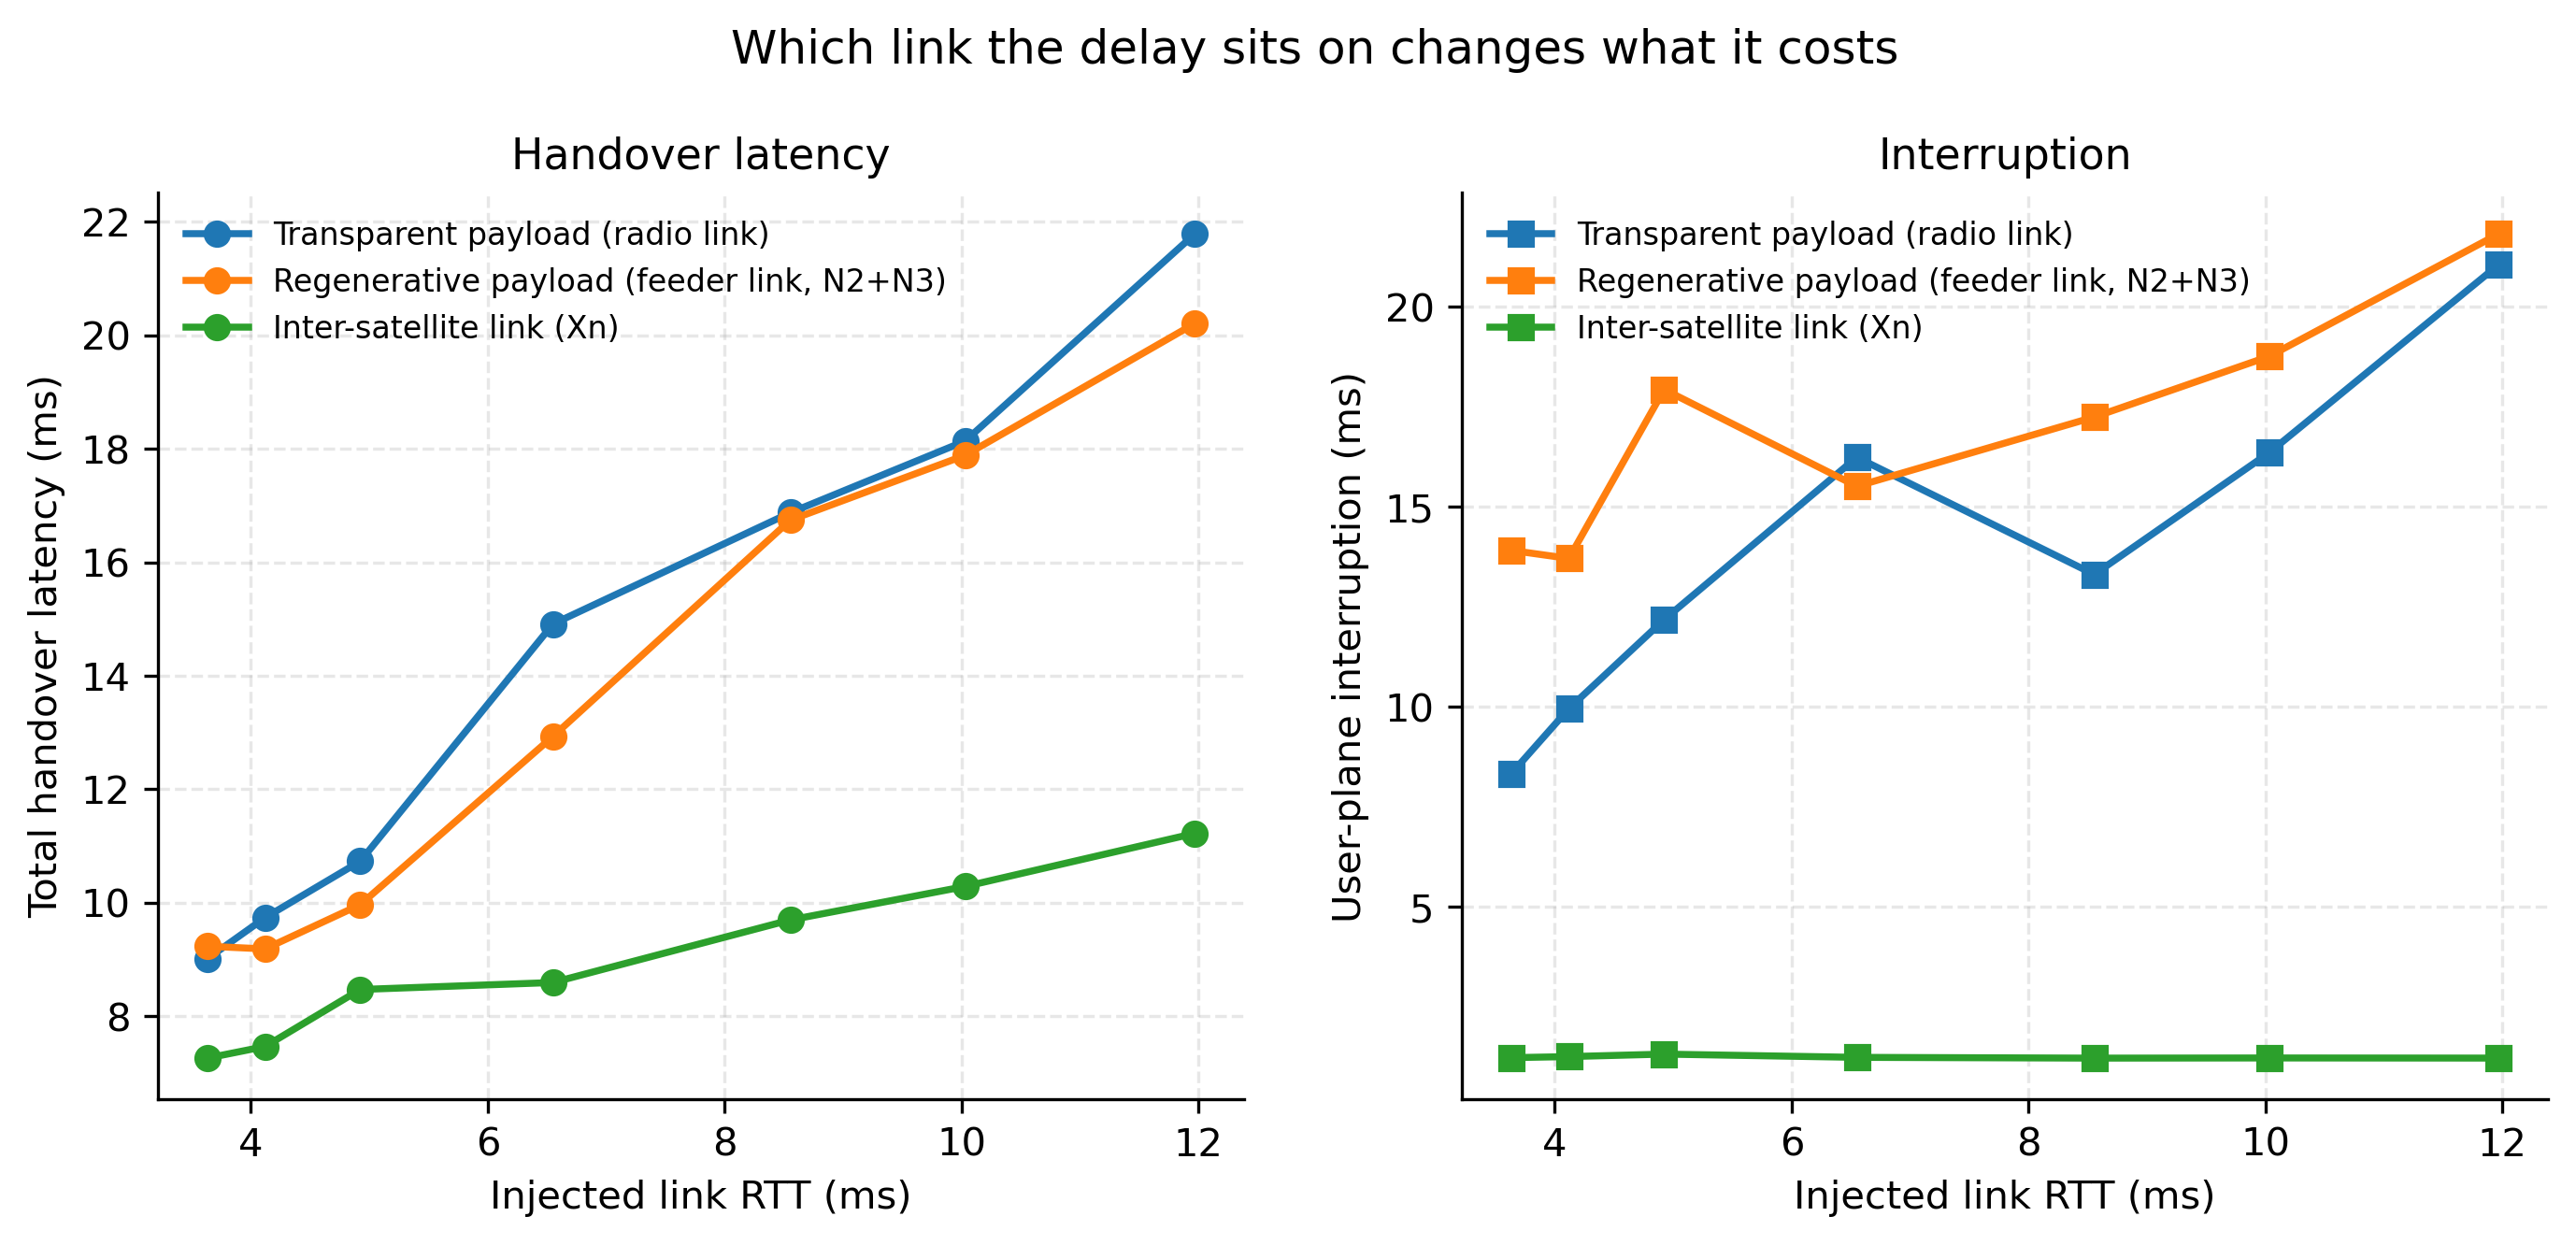
\includegraphics[width=0.86\textwidth]{fig_e2_comparison.png}
\caption{Handover latency (left) and user-plane interruption (right) against
injected link round-trip time. All architectures pay latency, but only those
whose delay is incurred after the UE leaves the source cell pay interruption.}
\label{fig:e2}
\end{figure*}

The results confirm the expected structure and isolate the asymmetry that
motivates this work.

Regenerative UE-arrival sensitivity is $+0.06$, i.e.\ flat: feeder delay does
not touch Xn signalling or the radio interface. Transparent UE-arrival
sensitivity is $+1.16 \approx 1$, consistent with the handover command
traversing the source radio link and the completion message traversing the
target link---one round trip in total. Inter-satellite path-switch sensitivity
is $-0.03$, i.e.\ zero: Xn delay genuinely does not touch the core round trip.

The inter-satellite UE-arrival slope of $+0.48$ deserves comment because it
appears wrong. One would expect $1.0$ for an Xn round trip. It is correct: the
measurement window opens when the target \emph{receives} the Handover Request,
so the request's own flight time falls outside it and only the acknowledgement
direction---one one-way hop, half a round trip---is captured. Obtaining $0.48$
rather than $1.0$ confirms the instrumentation measures the interval it claims.

The decisive result is the interruption column. Inter-satellite delay produces
$-0.01$\,ms of interruption per millisecond of link RTT: it is entirely free in
downtime terms, because the Xn exchange completes \emph{before} the UE is
instructed to move. Regenerative and transparent delay produce $+0.80$ and
$+1.24$ respectively, because they are incurred while the UE is between cells.
The same millisecond of propagation delay therefore costs radically different
amounts depending on which link carries it---a distinction invisible to
count-based analyses and directly actionable in constellation design and
satellite-selection optimisation.

One caveat bounds the transparent path-switch figure. Radio delay cannot
physically affect the gNB--AMF round trip, yet $+0.35$ is measured. Repeating
the scenario without probe traffic yields $-0.11$, identifying this as
measurement cross-talk rather than a property of the system.

\subsection{Policy Behaviour}

Evaluated offline against the real constellation schedule, the three policies
reproduce the trade-off documented in the literature. Maximum elevation performs
8 handovers per 15-minute window while maintaining a mean serving elevation of
$52.7^\circ$ (2.58\,ms mean delay). Both stability-focused policies perform 2,
at $25.9^\circ$ and $24.0^\circ$ respectively. The elevation-threshold policy
additionally produces a \emph{late} handover, in which the serving satellite is
lost before the switch fires---the known weakness of a fixed threshold, since
two passes may share an elevation while having very different remaining service
time. The maximum-service-time policy avoids this at equal handover count.

The resulting serving-elevation trajectories differ sharply. Maximum elevation
produces a characteristic sawtooth, abandoning satellites after a median of
1.3 minutes of a 7.4-minute pass---discarding roughly 80\% of each satellite's
usable service time---while the stability-focused policies retain each satellite
for approximately 6 minutes. These trajectories are visible per policy in
Fig.~\ref{fig:e4time}.

\subsection{Measured Cost of Policy Choice}
\label{sec:e4}

E4 executes those decisions against the live testbed, so each handover carries
its measured cost. Table~\ref{tab:e4} reports results over four independent
15-minute windows.

\begin{table}[t]
\caption{Measured policy cost, mean $\pm$ s.d.\ over four independent windows}
\label{tab:e4}
\centering
\begin{tabular}{lcccc}
\toprule
 & HO per & Cost per & Cumulative & Mean link \\
Policy & window & HO (ms) & outage (ms) & delay (ms) \\
\midrule
Max.\ elevation & 10.5 & $9.55 \pm 1.82$ & $97.5 \pm 16.7$ & 2.15 \\
Elev.\ threshold & 1.5 & $19.21 \pm 1.97$ & $26.4 \pm 12.2$ & 5.22 \\
Max.\ service time & 1.5 & $19.47 \pm 1.08$ & $29.1 \pm 16.7$ & 5.33 \\
\bottomrule
\end{tabular}
\end{table}

The central finding is in the second column. Handovers under the
maximum-service-time policy cost \emph{twice as much each} as those under
maximum elevation ($19.47$ vs.\ $9.55$\,ms). The reason is structural: a
policy that defers handover until the serving satellite is nearly setting
necessarily executes every handover across the longest, slowest links available.
The policy that minimises handover \emph{count} maximises handover \emph{cost}.

This materially changes the trade-off. On counts alone, maximum service time
appears $7\times$ better ($1.5$ vs.\ $10.5$ handovers). In measured cumulative
interruption the advantage is only $3.4\times$ ($29.1$ vs.\ $97.5$\,ms). Roughly
half the apparent benefit is consumed by the higher per-event cost.
Fig.~\ref{fig:e4frontier} presents this as the frontier an optimiser must trade
along, and Fig.~\ref{fig:e4time} shows the underlying pass sequences with
per-handover costs.

\begin{figure}[t]
\centering
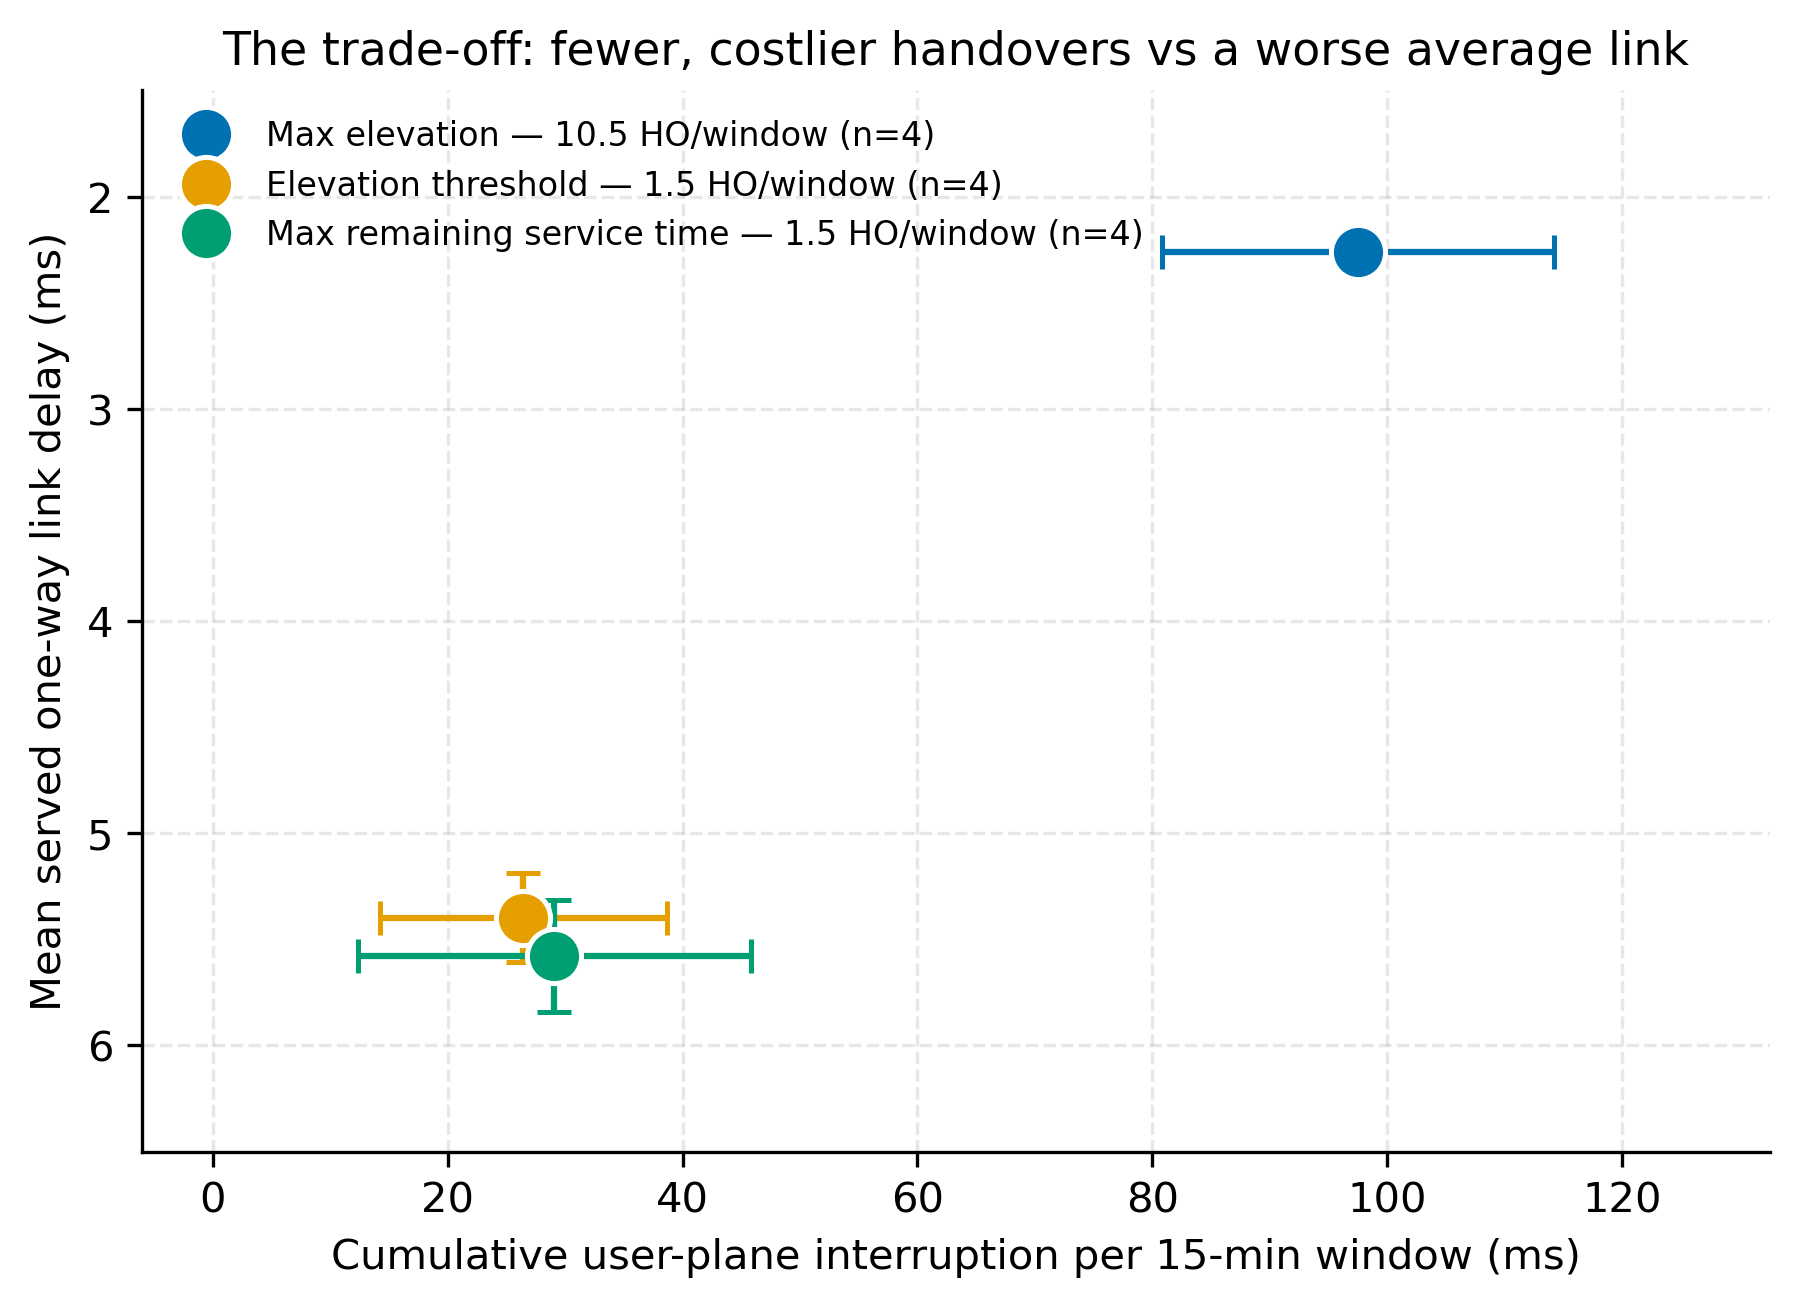
\includegraphics[width=\columnwidth]{fig_e4_frontier.png}
\caption{Measured trade-off between link quality and cumulative user-plane
interruption. Error bars span four independent 15-minute windows.}
\label{fig:e4frontier}
\end{figure}

\begin{figure*}[t]
\centering
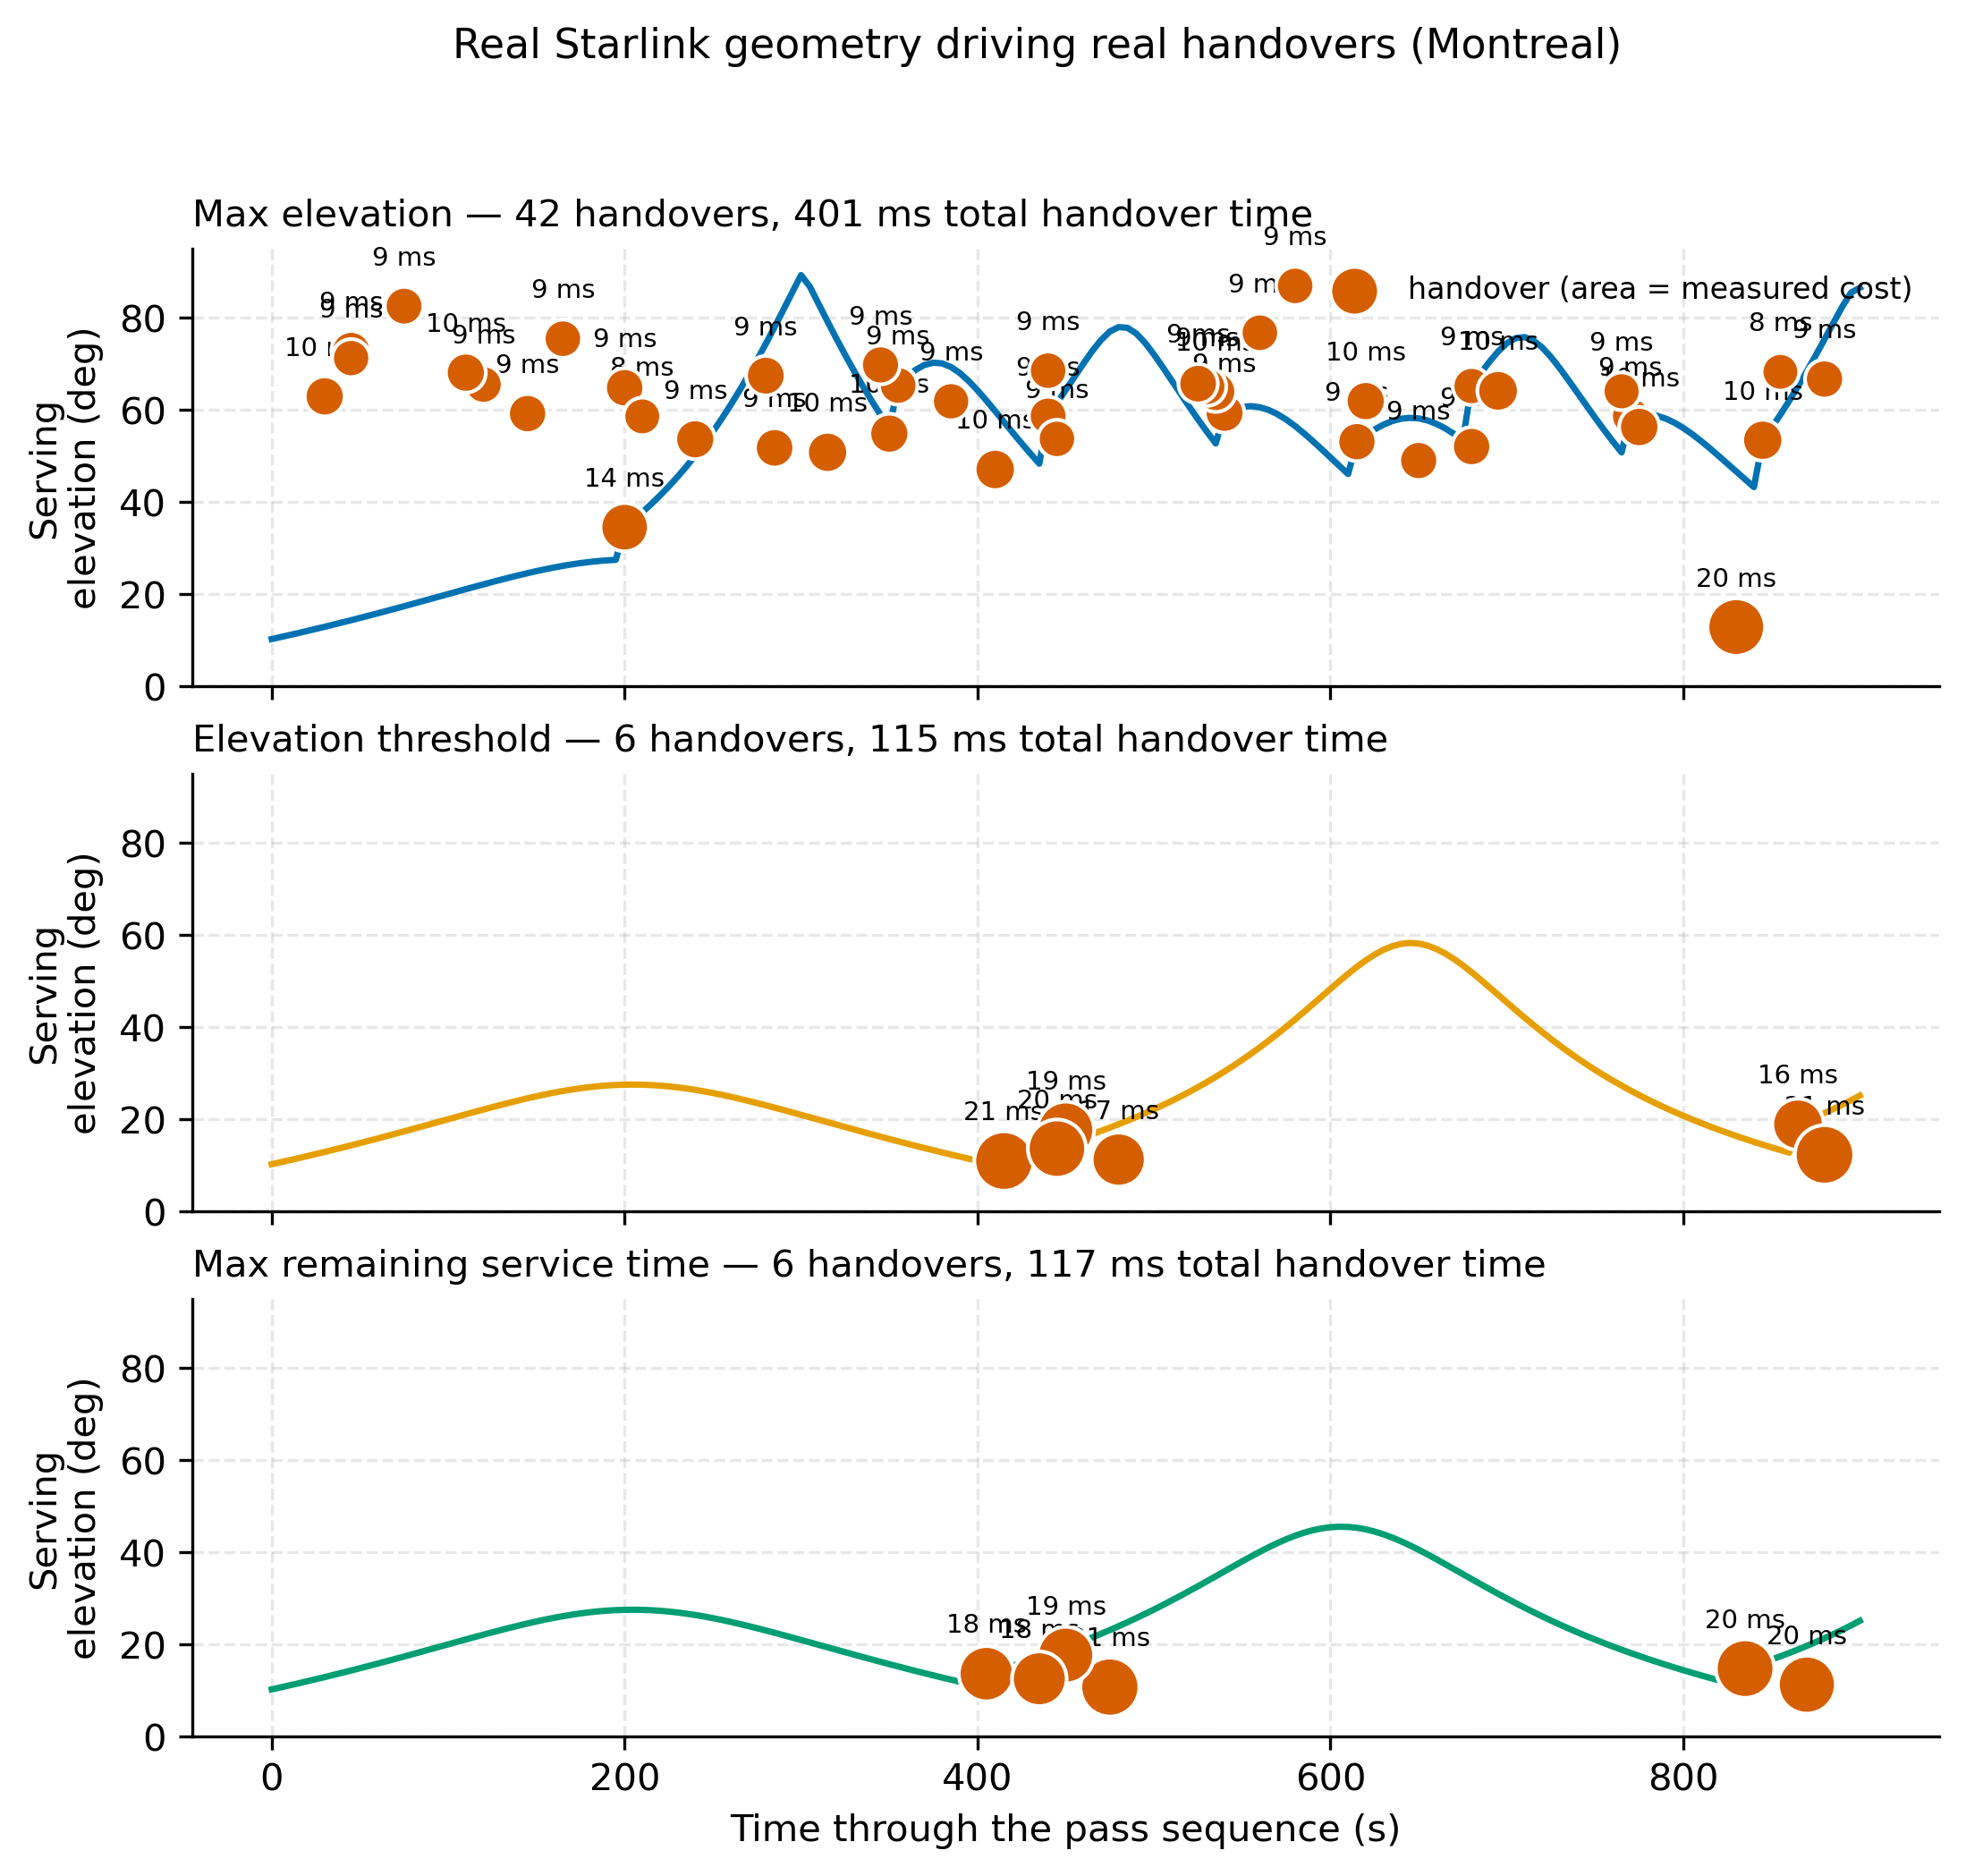
\includegraphics[width=0.80\textwidth]{fig_e4_timeline.png}
\caption{Real Starlink geometry driving real handovers. Marker area is
proportional to measured handover cost; low-elevation handovers are visibly more
expensive.}
\label{fig:e4time}
\end{figure*}

Fig.~\ref{fig:e4cost} makes the mechanism explicit: handover cost rises as the
elevation of the departing satellite falls, because both the source and target
links are longer.

\begin{figure}[t]
\centering
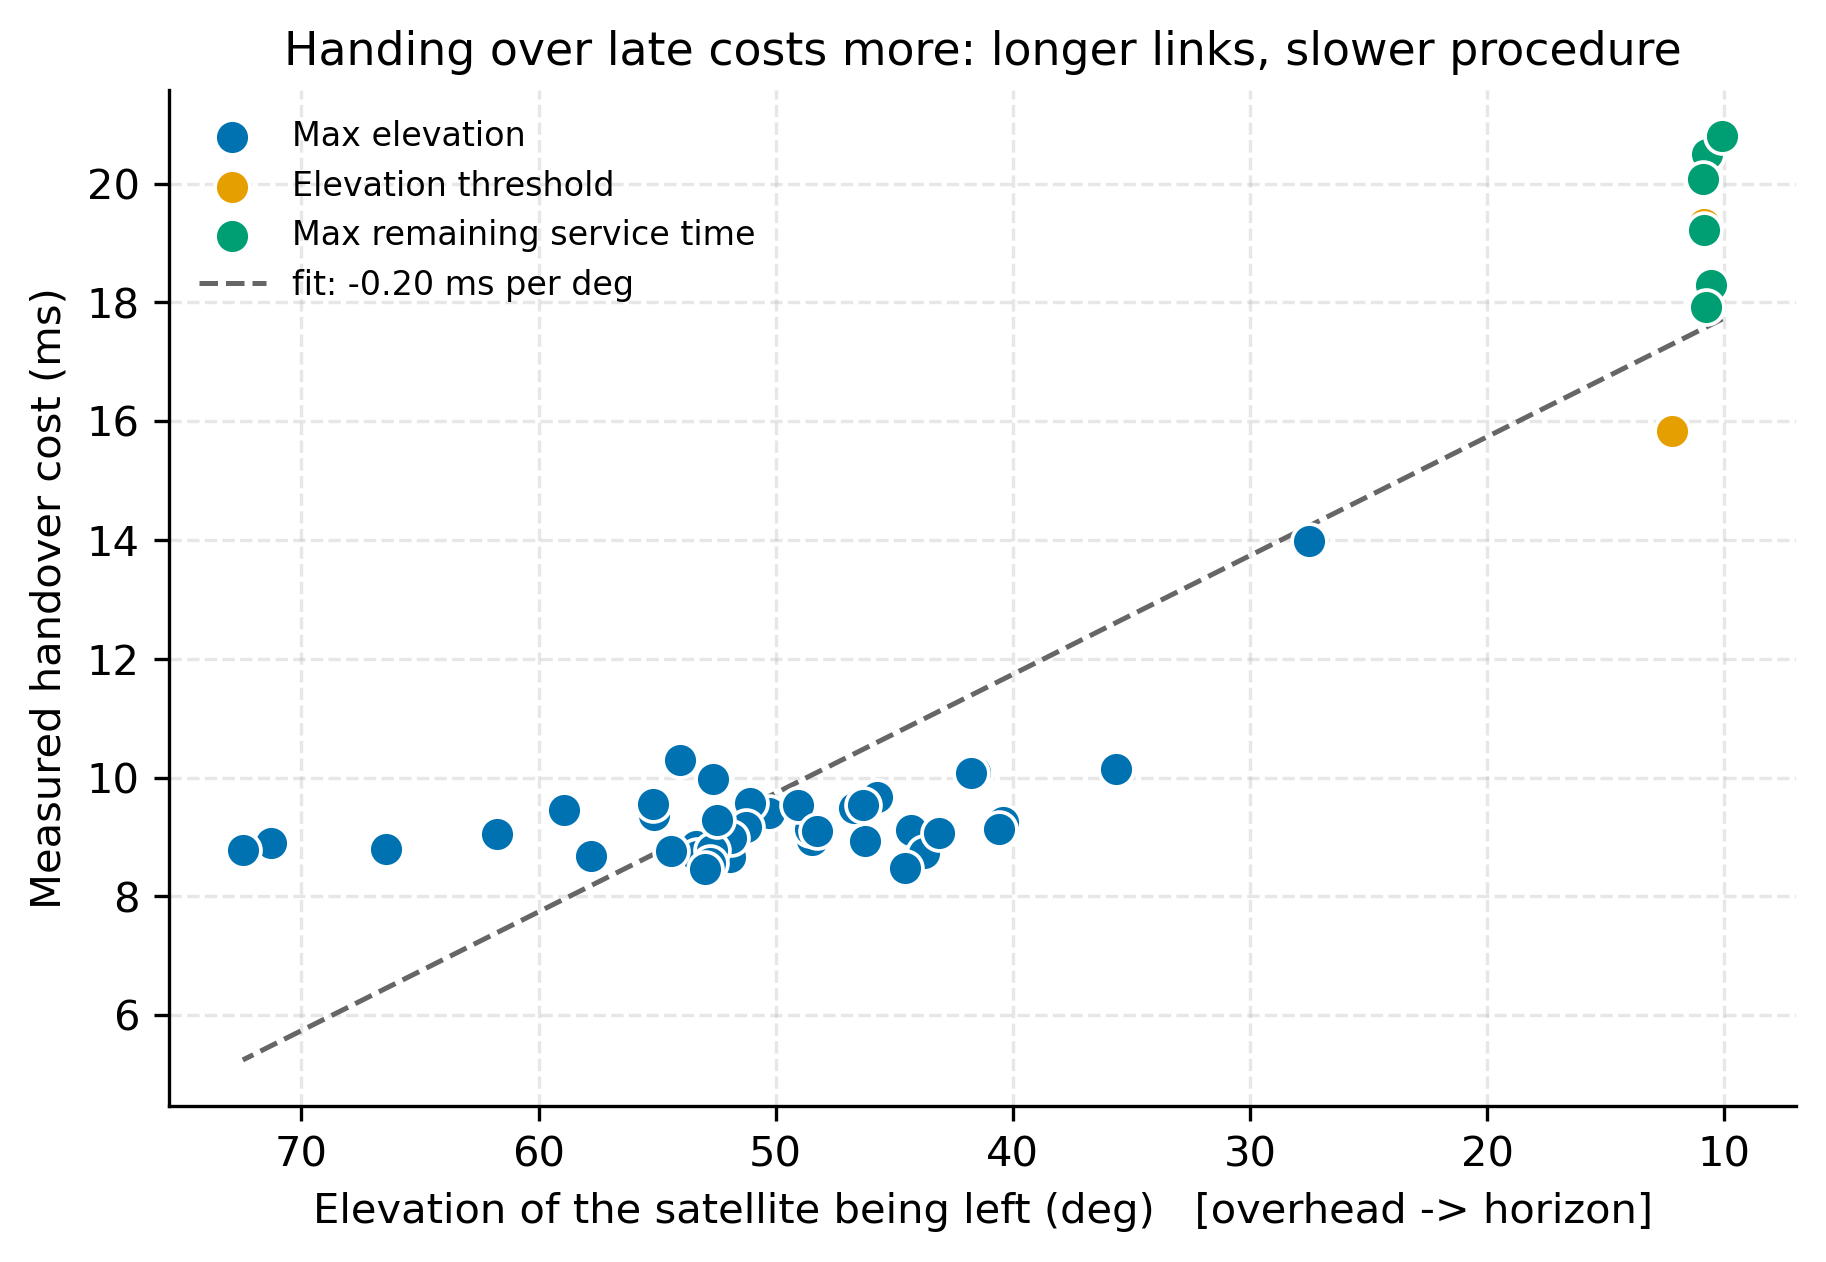
\includegraphics[width=\columnwidth]{fig_e4_cost_vs_elev.png}
\caption{Measured handover cost against the elevation of the satellite being
left. Handing over late is more expensive.}
\label{fig:e4cost}
\end{figure}

Repeating an identical window yields 78.5 versus 78.0\,ms cumulative cost for
maximum elevation (0.6\% difference) and 36.5 versus 37.0\,ms for the elevation
threshold (1.4\%), confirming reproducibility where the sample is adequate.

\section{Comparison with the Literature}

Our geometry agrees with published values: LEO one-way propagation delay is
reported as 1.6--6\,ms, against our ephemeris-derived 1.82--6.02\,ms. The
observation that a LEO satellite serves a user for only a few minutes is
consistent with our 7.4-minute median pass~\cite{ref_tutorial,ref_ntnperf}.

For policy behaviour the closest published comparison evaluates the same two
strategy families over 50 Monte Carlo runs \cite{ref_hybrid}, reporting 309.2
handovers for highest-elevation against 146.4 for longest-visibility---a 53\%
reduction---at a cost of 3.7\,dB in mean SINR. We observe an 86\% reduction at a
cost of $2.4\times$ in mean link delay. The direction, mechanism and qualitative
conclusion agree; our larger reduction is expected because our selection is
purely geometric, whereas SINR incorporates fading and antenna effects that
partly decouple from geometry. Related studies report reductions of 40--81\%
\cite{ref_demand,ref_optimal}, placing our figure just above a well-populated
range. That work states the trade-off explicitly---strategies maximising
instantaneous link quality trigger excessive handovers, while stability-focused
approaches sacrifice link performance---which is the frontier we measure.

Our interruption values (8--22\,ms) are below published handover interruption
times (${\sim}$35\,ms intra-gNB, $\geq$45\,ms LTE, 24/7.4\,ms NR FR1/FR2). This
is by construction, not by improvement: the testbed has no physical layer, and
the literature attributes 10\,ms to UE RRC processing alone. Our figures should
be read as the \emph{network-side contribution}, with radio-layer terms excluded.

What we did not find in the literature is any measurement of \emph{which link's}
delay converts into interruption, nor of per-handover cost as a function of
policy. Both follow from the 3GPP procedure ordering and are therefore
unsurprising once stated; the contribution is their quantification.

\section{Limitations}

The testbed has no physical layer: no random access, no timing advance, no
Doppler, fading or beam modelling. Absolute interruption times are consequently
lower bounds representing signalling and core processing only. A useful
consequence is that the emulated handover is inherently RACH-less, which aligns
with the NTN model rather than the terrestrial one, but timing-advance
pre-compensation cannot be represented.

The policy layer assumes exact geometry knowledge, consistent with the Rel-17
mandate for GNSS-capable NTN UEs, but ephemeris staleness and GNSS error are not
modelled. Delay is injected as a constant per link during each handover, which
is sound given that geometry evolves over minutes while a handover completes in
milliseconds, but does not capture continuous variation within a procedure.

Interruption resolution is one probe interval---1.2\,ms undelayed, 5--8\,ms
under injected delay---because probe pacing degrades toward the round-trip rate.
Outages below this cannot be distinguished from zero. Finally, the two
stability-focused policies overlap within error on both frontier axes with six
handovers each, so we report them as equivalent rather than ranked.

We also note one unresolved observation: for the inter-satellite scenario the
measured outage is consistently one probe interval, shorter than the path-switch
window would suggest. We hypothesise that the asynchronous serving-cell update
briefly preserves the old path, but have not verified this, and therefore make
no precise claim about absolute interruption in that scenario.

\section{Conclusion}

We measured the cost of 3GPP Xn handover under NTN propagation conditions using
an emulation testbed driven by real Starlink ephemeris. Across 470 handovers we
showed that delay on the inter-satellite Xn link inflates handover latency but
produces no user-plane interruption, because it is incurred before the UE
leaves the source cell, whereas feeder- and service-link delay convert almost
directly into downtime. Replaying real pass sequences, we showed that
per-handover cost is inversely related to handover frequency, so that counting
handovers overstates the benefit of stability-focused policies by roughly a
factor of two: the handovers such policies avoid are precisely the cheap ones.

These coefficients are directly usable in constellation and mobility
optimisation, where the relevant question is not how many handovers a policy
incurs but how much service time they consume. Extending the testbed with a
physical-layer model, and with data forwarding for lossless handover, would
allow the absolute figures to be compared against over-the-air measurements.

\begin{thebibliography}{00}

\bibitem{ref_38300} 3GPP, ``NR; Overall description; Stage-2,''
TS 38.300, 3rd Generation Partnership Project.

\bibitem{ref_38331} 3GPP, ``NR; Radio Resource Control (RRC) protocol
specification,'' TS 38.331, 3rd Generation Partnership Project.

\bibitem{ref_daps} ``5G NR Dual Active Protocol Stack (DAPS) Handover ---
3GPP Release 16,'' Techplayon. [Online]. Available:
\url{https://www.techplayon.com/5g-nr-dual-active-protocol-stack-daps-handover-3gpp-release-16/}

\bibitem{ref_ntnproc} ``5G NTN: Network Procedures and Parameters,''
nxgconnect. [Online]. Available:
\url{https://www.nxgconnect.com/post/5g-ntn-network-procedures-and-parameters}

\bibitem{ref_hybrid} ``A Low-Complexity Hybrid Handover Strategy for LEO NTN:
Balancing Stability and Link Quality,'' \emph{Sensors}, 2025. [Online].
Available: \url{https://pmc.ncbi.nlm.nih.gov/articles/PMC12987173/}

\bibitem{ref_demand} T.~Ahmed \emph{et al.}, ``Demand-aware Flexible Handover
Strategy for LEO Constellation,'' in \emph{Proc. IEEE ICC}, 2023.

\bibitem{ref_optimal} ``Optimal Handover Strategies in LEO Satellite
Networks,'' arXiv preprint arXiv:2512.02449.

\bibitem{ref_graph} ``A Graph-Based Customizable Handover Framework for LEO
Satellite Networks,'' arXiv preprint arXiv:2211.07872.

\bibitem{ref_tutorial} ``A Tutorial on Non-Terrestrial Networks: Towards Global
and Ubiquitous 6G Connectivity,'' arXiv preprint arXiv:2412.16611.

\bibitem{ref_ntnperf} ``On the Performance of Handover Mechanisms for
Non-Terrestrial Networks,'' arXiv preprint arXiv:2201.04904.

\bibitem{ref_open5gs} Open5GS. [Online]. Available: \url{https://open5gs.org/}

\bibitem{ref_ueransim} UERANSIM. [Online]. Available:
\url{https://github.com/aligungr/UERANSIM}

\bibitem{ref_skyfield} B.~Rhodes, ``Skyfield: High precision research-grade
positions for planets and Earth satellites.'' [Online]. Available:
\url{https://rhodesmill.org/skyfield/}

\end{thebibliography}

\balance
\end{document}
